\section{Data retrieval process: gather and formatting social media data}

In this work it is proposed three datasets with social data from three social networks that are Twitter, Reddit and post blogs. Each dataset is build by using three different APIs: the Twitter API for the Twitter dataset, the Twingly API for the blog posts dataset and the Social Searcher API for the Reddit dataset. For each dataset it is considered a set of keywords that will retrieve social information by exact matching within corpus of each document. Since the retrieval must be performed for different languages, the keywords corresponds to named entities or specific lingo used in the social media in question in order to execute retrieval queries whose words do not need to be translated to the target language. As it will be seen, some tweets were retrieved by using the special character \textit{\$} which denotes information related to the stock market.

\par The next sections are intended to explain the gathering process, how the data is formatted in order to persist it according to legal concerns of the social media source information and some limitations related to the use of these type of APIs and the information they provide.
\subsection{Gathering process}
%APIS: Twitter, Twingly and Social Media Searcher
Typically, in the gathering process of any type of social data is implied the time variable which, for example,  can be used to cluster documents by fixed window times. The building process of the different datasets provided comprise periods of time in terms of its retrieval. The Table \ref{table:periodTime} shows the dates when the retrieval process starts and ends per dataset.

\begin{table}[htb]
	\begin{center}
		\begin{tabular}{|l|r|r|}
			\hline
			\textbf{Dataset} &    \textbf{Start date } &\textbf{ End date}\\
			\hline \hline
			Twitter              &  2021-12-04  &  2021-12-31\\ 
			\hline
			Blog posts &  2021-11-08 	& 2021-12-06 \\
			\hline
			Reddit &  2021-11-08   	& 2021-12-06 \\
			\hline
		\end{tabular}
	\end{center}
	\caption{Start and end dates of the retrieval data}
	\label{table:periodTime}
\end{table}

Each dataset is built according to a fixed set of keywords that corresponds to named entities. Each keyword belongs to the domain of music, stock market, news related to a natural disaster, technology and influencers. Each keyword corresponds with a named entity. The Table \ref{table:keywords} summarizes this information.\\

%Social media considered, Keywords (named entities), gathering time window.
\begin{table}[H]
	\centering
	\begin{tabular}{|c|c|c|c|c|}
		\hline
		\textbf{Keyword} & \textbf{Domain} & \multicolumn{3}{c|}{\textbf{Dataset}} \bigstrut\\
		\hline \hline
		\textit{paramore} & \multirow{3}[6]{*}{Music} & \multirow{14}[28]{*}{Twitter} & \multirow{7}[14]{*}{Blog posts} & \multirow{6}[12]{*}{Reddit} \bigstrut\\
		\cline{1-1}    \textit{my chemical romance} &       &       &       &  \bigstrut\\
		\cline{1-1}    \textit{the smashing pumpkins} &       &       &       &  \bigstrut\\
		\cline{1-2}    \textit{la palma} & News  &       &       &  \bigstrut\\
		\cline{1-2}    \textit{dalas} & Influencer &       &       &  \bigstrut\\
		\cline{1-2}    \textit{apple} & \multirow{2}[4]{*}{Technology} &       &       &  \bigstrut\\
		\cline{1-1}\cline{5-5}    \textit{microsoft} &       &       &       & \multirow{8}[16]{*}{} \bigstrut\\
		\cline{1-2}\cline{4-4}    \textit{\$AMC} & \multirow{7}[14]{*}{Financial} &       & \multirow{7}[14]{*}{} &  \bigstrut\\
		\cline{1-1}    \textit{\$GME} &       &       &       &  \bigstrut\\
		\cline{1-1}    \textit{\$AAPL} &       &       &       &  \bigstrut\\
		\cline{1-1}    \textit{\$HOOD} &       &       &       &  \bigstrut\\
		\cline{1-1}    \textit{\$MSFT} &       &       &       &  \bigstrut\\
		\cline{1-1}    \textit{\$NVDA} &       &       &       &  \bigstrut\\
		\cline{1-1}    \textit{\$TWKS} &       &       &       &  \bigstrut\\
		\hline
	\end{tabular}%
	\caption{Keywords with their domain and datasets containing them.}
	\label{table:keywords}%
\end{table}%
\par 
The intention for each dataset is to be multilingual in order to analyze differences between the datasets and the named entities in function of the language. Hence, seven languages are proposed in the retrieval process that are English, Spanish, French, Portuguese, Italian German and Dutch.
For each day in the periods of time described in Table \ref{table:periodTime} a daily retrieval process was executed. For the Twitter dataset, it was retrieved 100,000 tweets per day. The blog posts dataset was built only with a single API call since Twingly indexes articles and stores them in their database and the API call retrieves information persisted from the three last months. However, for the Reddit dataset only 100 posts could be retrieved per day. All the datasets were filtered in order to delete repeated posts.
\subsection{Formatting process}
The three APIs used to retrieve the social data define a set of properties returned in the response of the API call. However, not all information is considered in the dataset building process for legal or practical reasons. In the gathering and processing the Twitter information the textual information must be deleted because the Twitter terms and conditions of its API usage. It is important to remark that with the tweet ID or the user ID it can be retrieved more information provided by the Twitter API. In this work, it will be only considered these IDs and the date and language of each tweet. The following schema defines the structure of a tweet in the dataset.
%Tweet
\begin{figure}[H]
	\begin{Verbatim}[xleftmargin=.5in]
		// Tweet format
		{
			"date": ,
			"id_tweet": ,
			"language": ,
			"user_id": 
		}
	\end{Verbatim}
	\caption{Structure of a retrieved tweet.}
\end{figure}


\par 

The Reddit dataset contains information about the sentiment of the text and popularity information related to the number of likes and comments of each post. the Figure \ref{fig:twinglyStructure} shows the schema for a persisted Reddit post in the dataset.
\begin{figure}[H]
	\begin{Verbatim}[xleftmargin=.5in]
		{
			// Reddit document format
			"post_id": ,
			"lang": ,
			"date_posted": ,
			"sentiment": ,
			"text": ,
			"ups": ,
			"comments": ,
			"user_name": ,
			"user_id": ,
			"user_url": 
		}
	\end{Verbatim}
	\caption{Structure of a Reddit post.}
	\label{fig:redditStructure}
\end{figure}

\par

Lastly, the Twingly API was used to retrieve the blog posts information regarding the keywords and languages considered. In comparison with the later structures, Twingly provides more information like the images attached for each post or the links contained in it. The blog post structure is depicted in the Figure \ref{fig:twinglyStructure}.
%Blog posts
\begin{figure}[H]
	\begin{Verbatim}[xleftmargin=.5in]
		// Blog post document format
		{
			"author": ,
			"authority": ,
			"blog_id": ,
			"blog_name": ,
			"blog_rank": ,
			"blog_url": ,
			"coordinates": ,
			"id": ,
			"images": ,
			"indexed_at": ,
			"inlinks_count": ,
			"language_code": ,
			"latitude": ,
			"links": ,
			"location_code": ,
			"published_at": ,
			"reindexed_at": ,
			"tags": ,
			"text": ,
			"title": ,
			"url"
		}
	\end{Verbatim}
	\caption{Structure of a blog post}
	\label{fig:twinglyStructure}
\end{figure}
\subsection{Limitations}

The Twitter API limits the number of API calls per day. This led to the retrieval process to take several hours because wait clauses must be coded to avoid the rejection of API calls by the Twitter side. Furthermore, the textual information can not be shared publicly due to legal Twitter concerns. However, with the tweet ID it is possible to retrieve the metadata that defines a tweet such that the geographical position where the tweet was posted, the number of retweets etc. \\

\par Twingly provides a great API to retrieve blog posts. However, the supported format is XML which is not the trend nowadays. Nonetheless, there exists packages that allow to translate files from XML to JSON format.
\par Lastly, the Social Searcher API is the most restrictive. Only 100 posts per API call can be retrieved and the language of the posts is not guaranteed to match with the one specified in the API call. However, the API response contains attributes that can be exploited in the sentiment analysis context like the sentiment property.
%Reddit


\section{Data analysis}

Mining information from social data is not a trivial task since there are some aspects that must be taken into account. First the noise data will difficult the execution of Machine Learning algorithms, noise that is mostly related to misspellings. Secondly the lack of textual data in the microblogging sites obstructs the application of these algorithms. This motivates to enrich the dataset with external sources like Wikipedia \citep{wikiEnrichTwitter} or with the links that can potentially contain.
\par However, in this work it will be assessed the question of what type of data is likely to be used in further analyses and what tools covers the variables considered in this study. For example, exclude those languages that do not contain enough information to train Machine Learning models or exploit determined attributes to enrich the textual information. For this, two analyses are proposed at different levels of granularity: (1) At dataset level where it is depicted some statistics related to the languages and the dates when the social data was posted; (2) At named entity level where it is studied whether some specific lingo for a given dataset could be used in these potential analyses.


\subsection{Analysis at dataset level}
For the analysis at dataset level it will be considered two common variables across the three datasets: the language and the number of posts per date.
\subsubsection{Twitter dataset analysis}
The figure \ref{fig:twitter_postcounts_date} shows top 100 dates ordered by the number of tweets published. This suggests an analysis of the tweets posted those days in order to detect sudden events.
However, the Twitter dataset is the largest one and cannot be compared with the other at first glance.
\begin{figure}[H]
	\begin{center}
		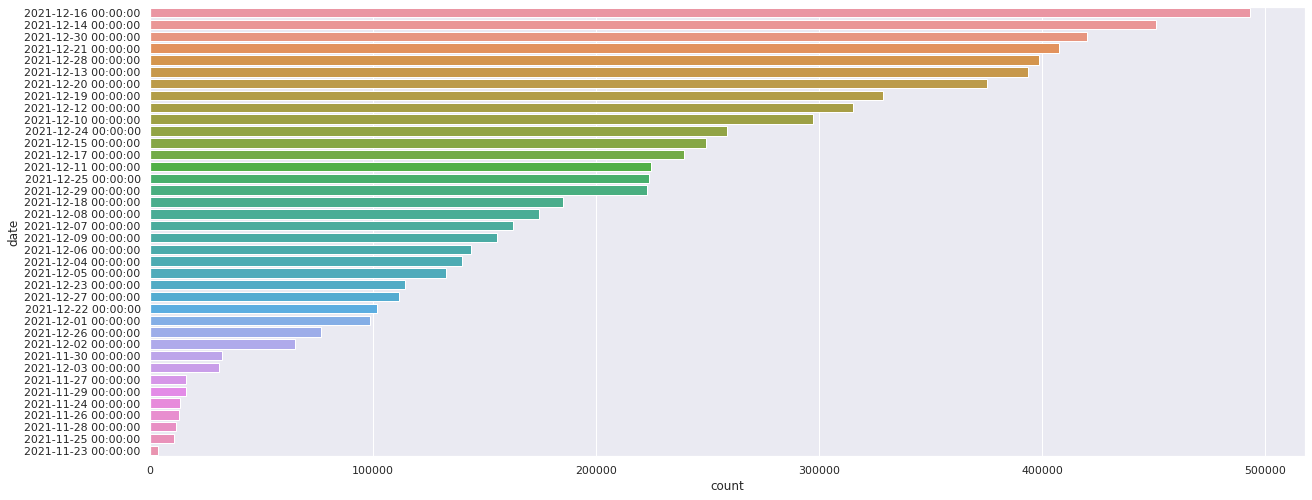
\includegraphics[scale=0.33]{twitter/datasetlevel/twitter_postcounts_date.png}
		\caption{Number of tweets published per date. Only the dates with higher values are shown.}
		\label{fig:twitter_postcounts_date}
	\end{center}
\end{figure}

\par For the language categorical variable, the count of tweets of each value is shown in the Figure \ref{fig:twitter_postcounts_lang}. Since there is more available data for the English language, it is feasible to study a specific task with a monolingual approach an then tackle the problem but with a multilingual perspective. However, when the task becomes multilingual it must be taken into account that the NLP tools are limited for certain languages. CoreNLP provides a pipeline to tokenize, perform a PoS tagging, lemmatize and detect named entities given a document for multiples languages \citep{coreNlp}. 
\par In the case of Twitter the challenges not only appears from the multilingual side. Deal with short texts with misspellings makes tougher Machine Learning tasks like clustering or classification since the lack of data and the noise will affect in the performance of the trained model in terms of their prediction capability. An approach to avoid this issue could be to retrain the current models in order to adapt them to the nuances of the tweet data \citep{synthesisLecturesSocial}. However, this probably will lead to models trained over these specific features and the desired generalization of the retrained models will not be guaranteed. This fact motivates the design of systems that normalize the input text in order to reuse the trained models for the NLP tasks.
\begin{figure}[H]
	\begin{center}
		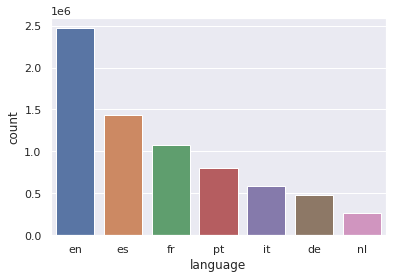
\includegraphics[scale=0.5]{twitter/datasetlevel/twitter_postcounts_lang.png}
		\caption{Tweet posts count per language.}
		\label{fig:twitter_postcounts_lang}
	\end{center}
\end{figure}
\subsubsection{Blog post dataset analysis}
The distribution of blog posts per language is quite similar to the Twitter dataset as shown in the Figure \ref{fig:blogpost_postcounts_lang}. Also, for the amount of posts published per date, there exists some days the number of posts soars.
\begin{figure}[H]
	\begin{center}
		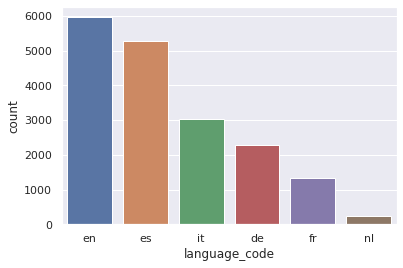
\includegraphics[scale=0.5]{blogposts/datasetlevel/blogpost_postcounts_lang.png}
		\caption{Blog posts count posted per language.}
		\label{fig:blogpost_postcounts_lang}
	\end{center}
\end{figure}

\begin{figure}[H]
	\begin{center}
		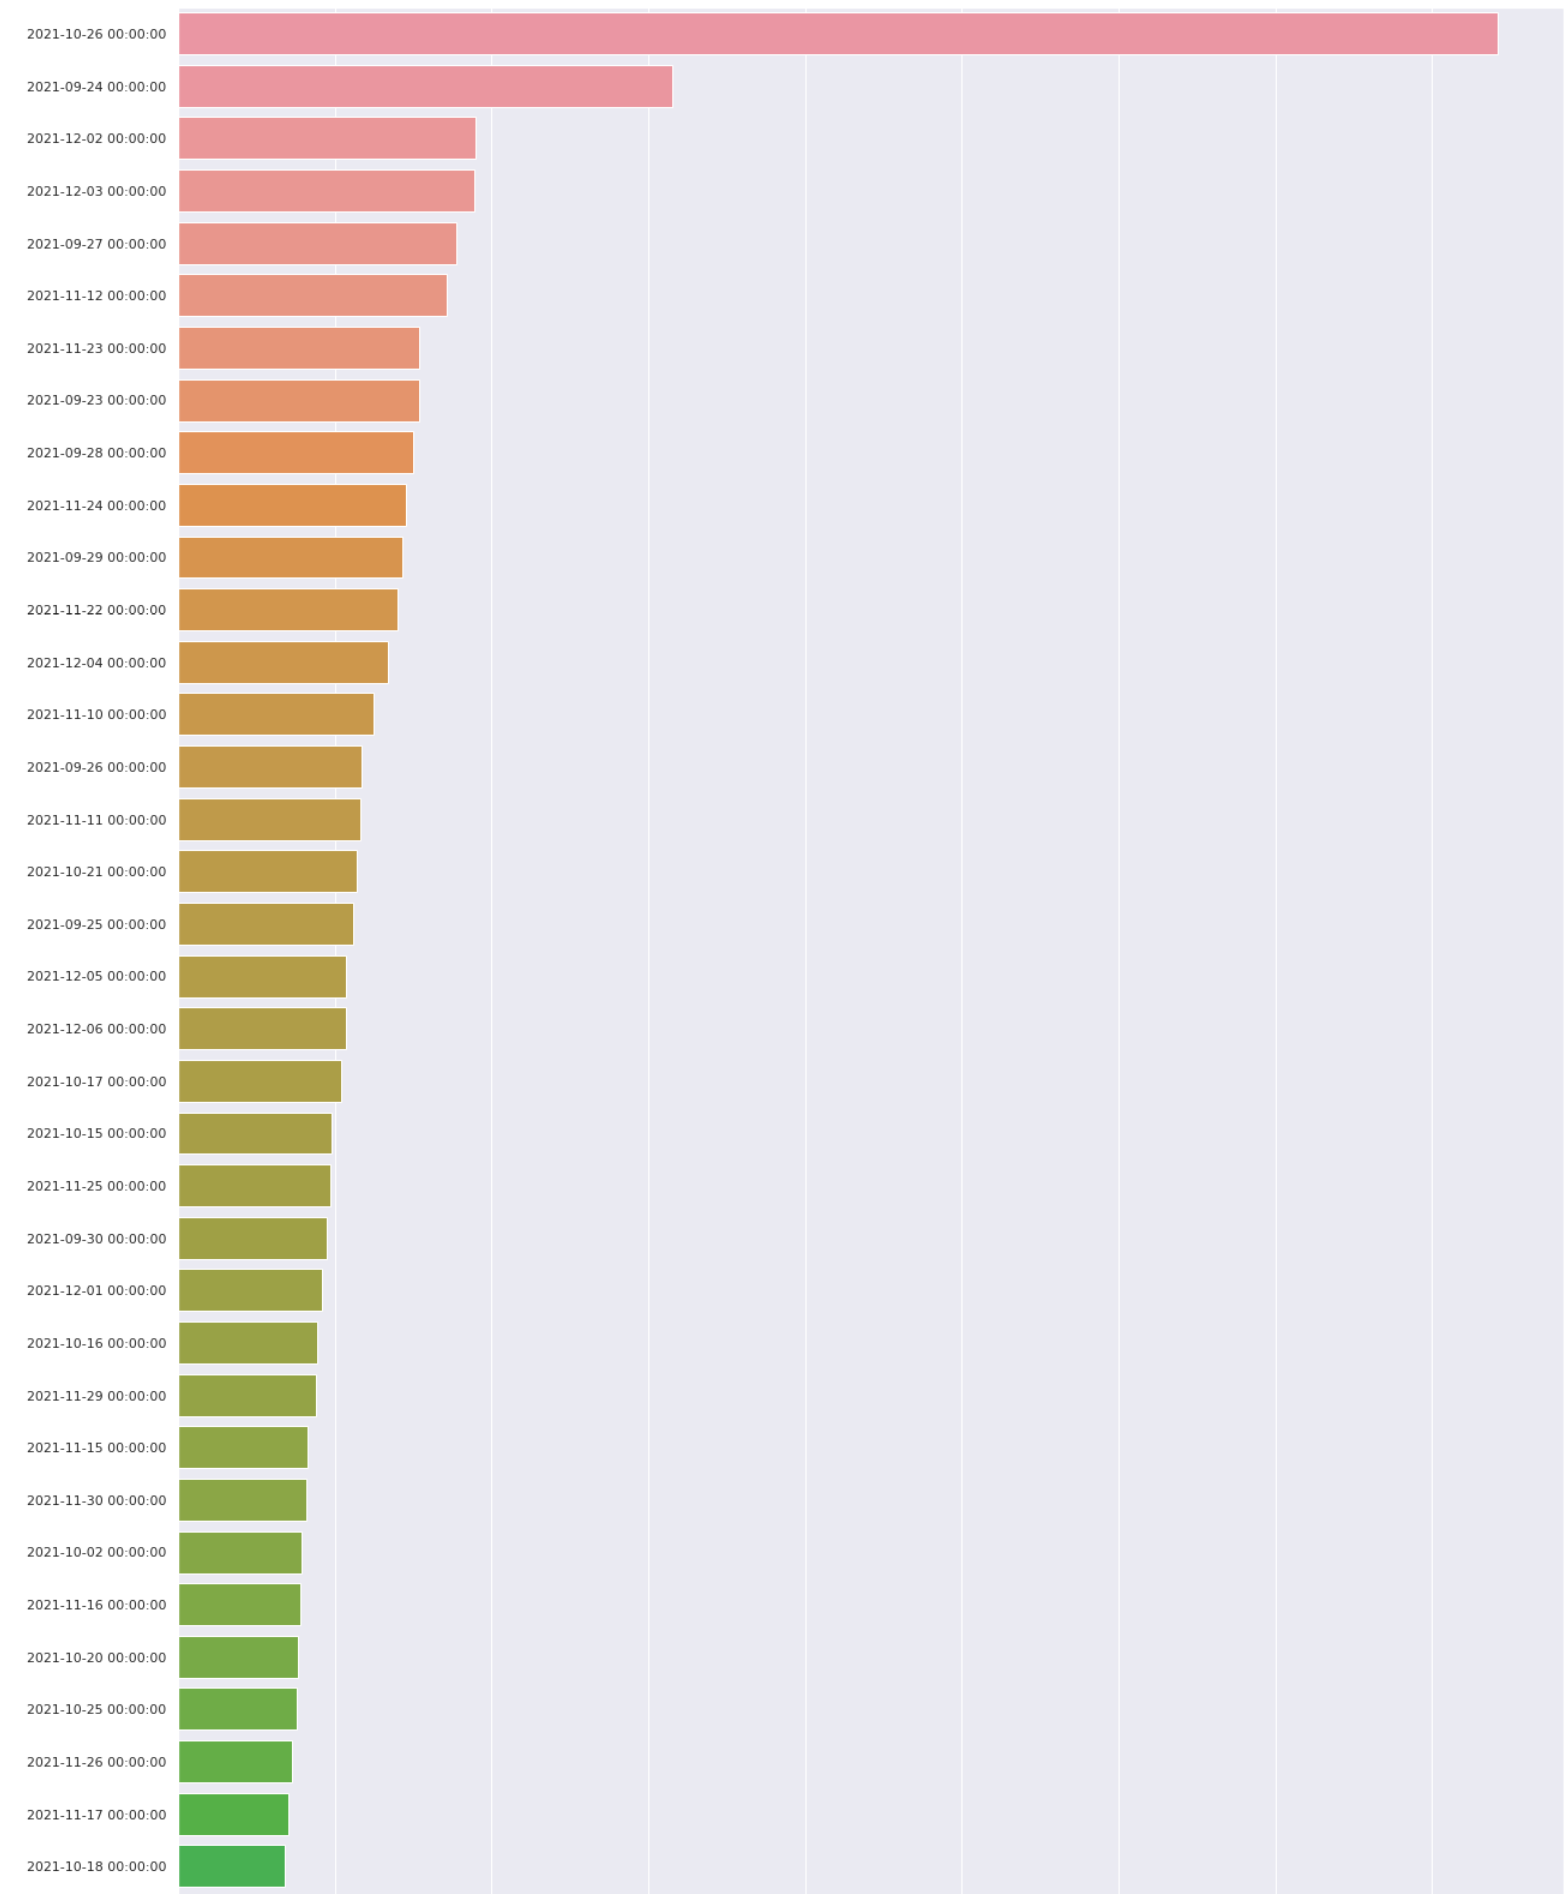
\includegraphics[scale=0.49]{blogposts/datasetlevel/blogpost_postcounts_date.png}
		\caption{Blog posts count posted per date. Only the dates with higher values are shown.}
		\label{fig:blogpost_postcounts_date}
	\end{center}
\end{figure}


\subsubsection{Reddit dataset analysis}
Something quite different occurs with the Reddit dataset. First of all, despite the predominant language is the English, there are fewer posts for the remaining languages. Furthermore, there are languages not reflected in the proposed ones. This is due issues of the Social Media Searcher API. Note that the total number of posts are fewer in comparison to the later datasets. The Figure \ref{fig:reddit_postcounts_lang} depicts the count of Reddit posts per language.

\begin{figure}[H]
	\begin{center}
		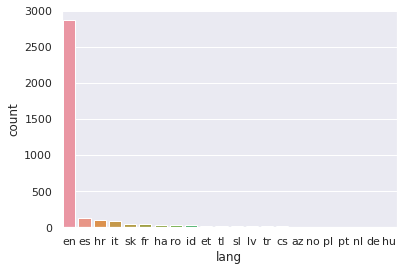
\includegraphics[scale=0.5]{reddit/datasetlevel/reddit_postcounts_lang.png}
		\caption{Reddit posts count posted per language.}
		\label{fig:reddit_postcounts_lang}
	\end{center}
\end{figure}

From the Figure \ref{fig:reddit_postcounts_date} it can be stated that, regardless the social data, the time variable could be used to mine information related to events by considering, for example, the hypothesis that posts with common words and published in similar dates will form clusters of related posts.
\begin{figure}[H]
	\begin{center}
		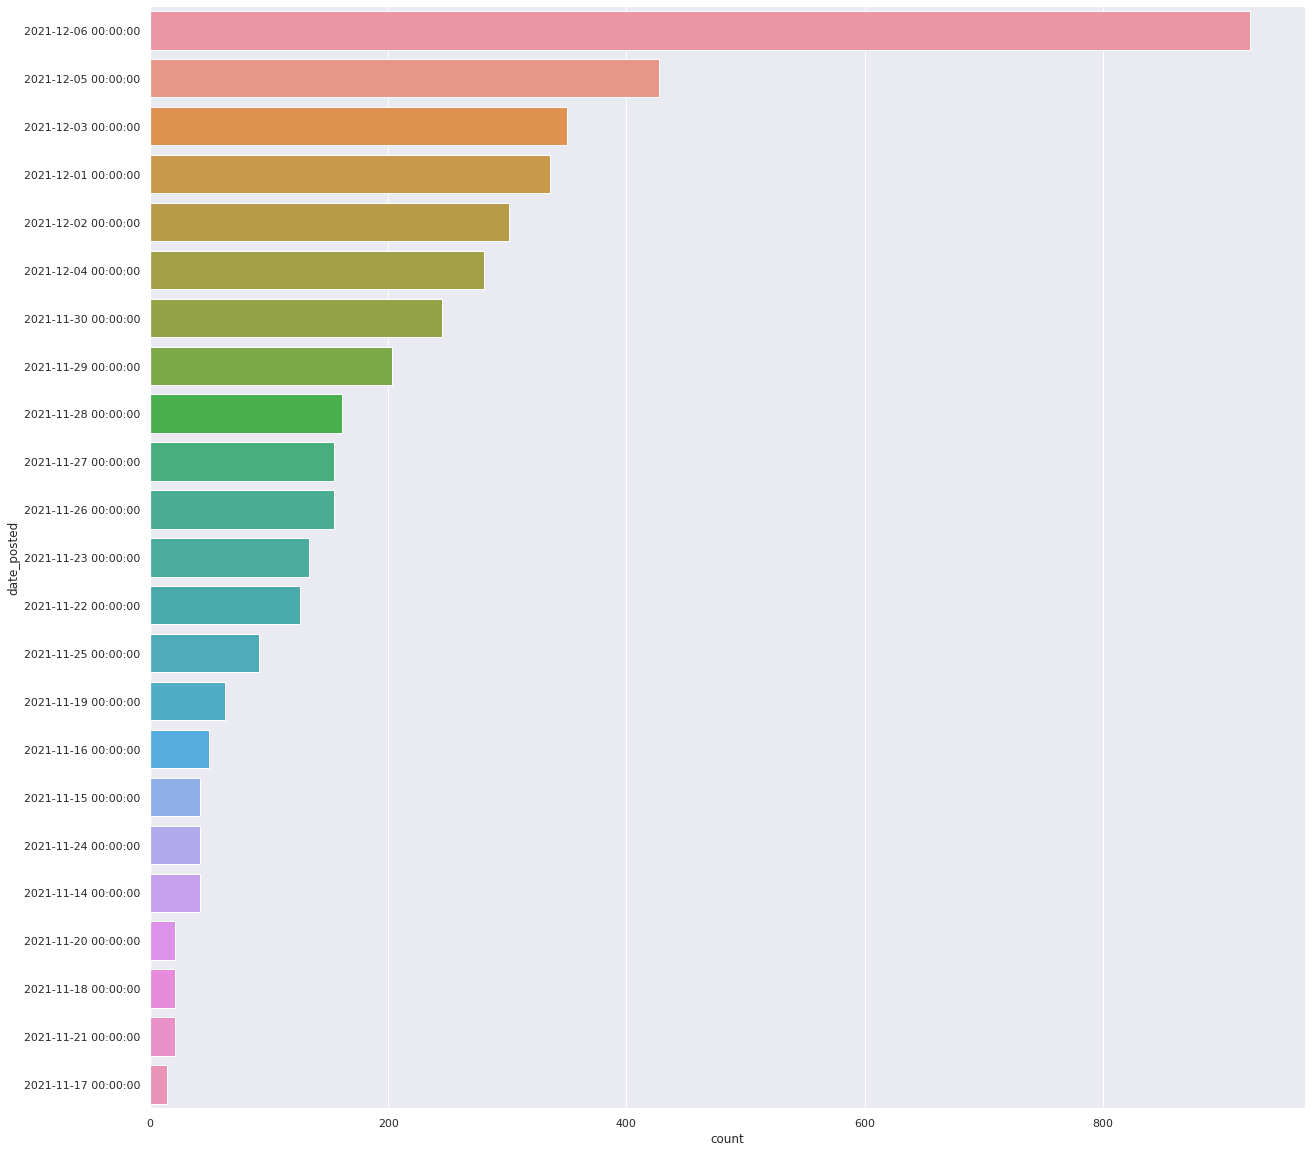
\includegraphics[scale=0.35]{reddit/datasetlevel/reddit_postcounts_date.png}
		\caption{Reddit posts count posted per date. Only the dates with higher values are shown.}
		\label{fig:reddit_postcounts_date}
	\end{center}
\end{figure}

% 

\subsection{Analysis at named entity level.}
This analysis is intended to elucidate variables that could be candidates to be considered in further analyses. This analysis will focus on specific features of the social media source for the different named entities considered.
%TODO
\subsubsection{Twitter named entity analysis}

The Figure \ref{fig:twitter_postcounts_entity} depicts the count of tweets per language and named entity. The Twitter dataset contains higher number of tweets for the \textit{covid} keyword and for each language considered. This fact could explain the uncertainty related to the average number of links per named entity as is shown in the Figure \ref{fig:twitter_average_links}.
\begin{figure}[H]
	\begin{center}
		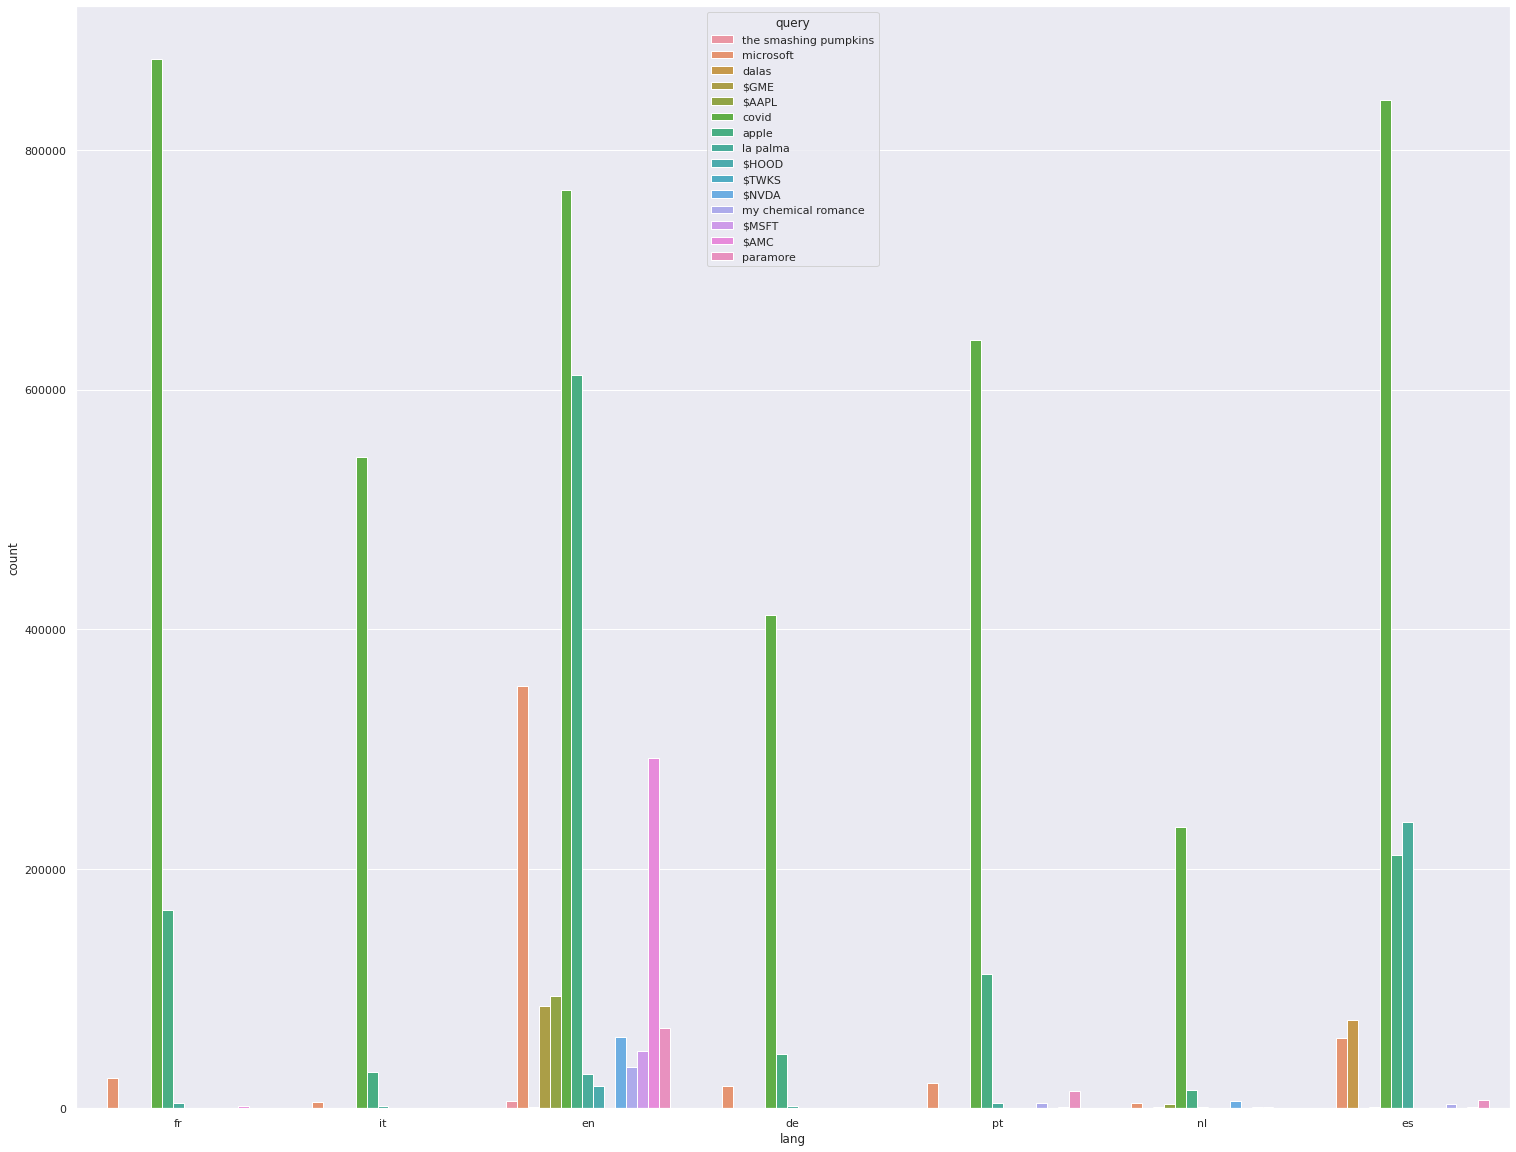
\includegraphics[scale=0.27]{twitter/namedentitylevel/twitter_postcounts_entity.png}
		\caption{Tweet posts count posted per language and named entity.}
		\label{fig:twitter_postcounts_entity}
	\end{center}
\end{figure}

The average number of links per named entity and the relatively low variance demonstrate that links could be a proper candidate to enrich, somehow, the tweet data with the content of the links and cover their inherent lack of information.
\begin{figure}[H]
	\begin{center}
		\includegraphics[scale=0.26]{twitter/namedentitylevel/twitter_average_\#links.png}
		\caption{Average number of links per named entity.}
		\label{fig:twitter_average_links}
	\end{center}
\end{figure}

\par A hashtag is a specific Twitter feature. Hashtags are intended to act as a summarization of the tweet in terms of the topic they cover. However, exploiting information from hashtags is a difficult task. First of all not all tweets will contain hashtags. The Figure \ref{fig:twitter_averagecount_hashtags} plots the average number of hashtags per named entity regardless the language. There are hardly any hashtags for the keyword \textit{dalas} in contrast with the keyword \textit{\$AMC} which reaches the maximum average amongst the remaining keywords. However, it is important to highlight that the maximum average is 0.75 approximately and the average number of hashtags per named entity is, in general, small. Therefore, it is expected that there will be tweets that do not contain a hashtag.

\begin{figure}[H]
	\begin{center}
		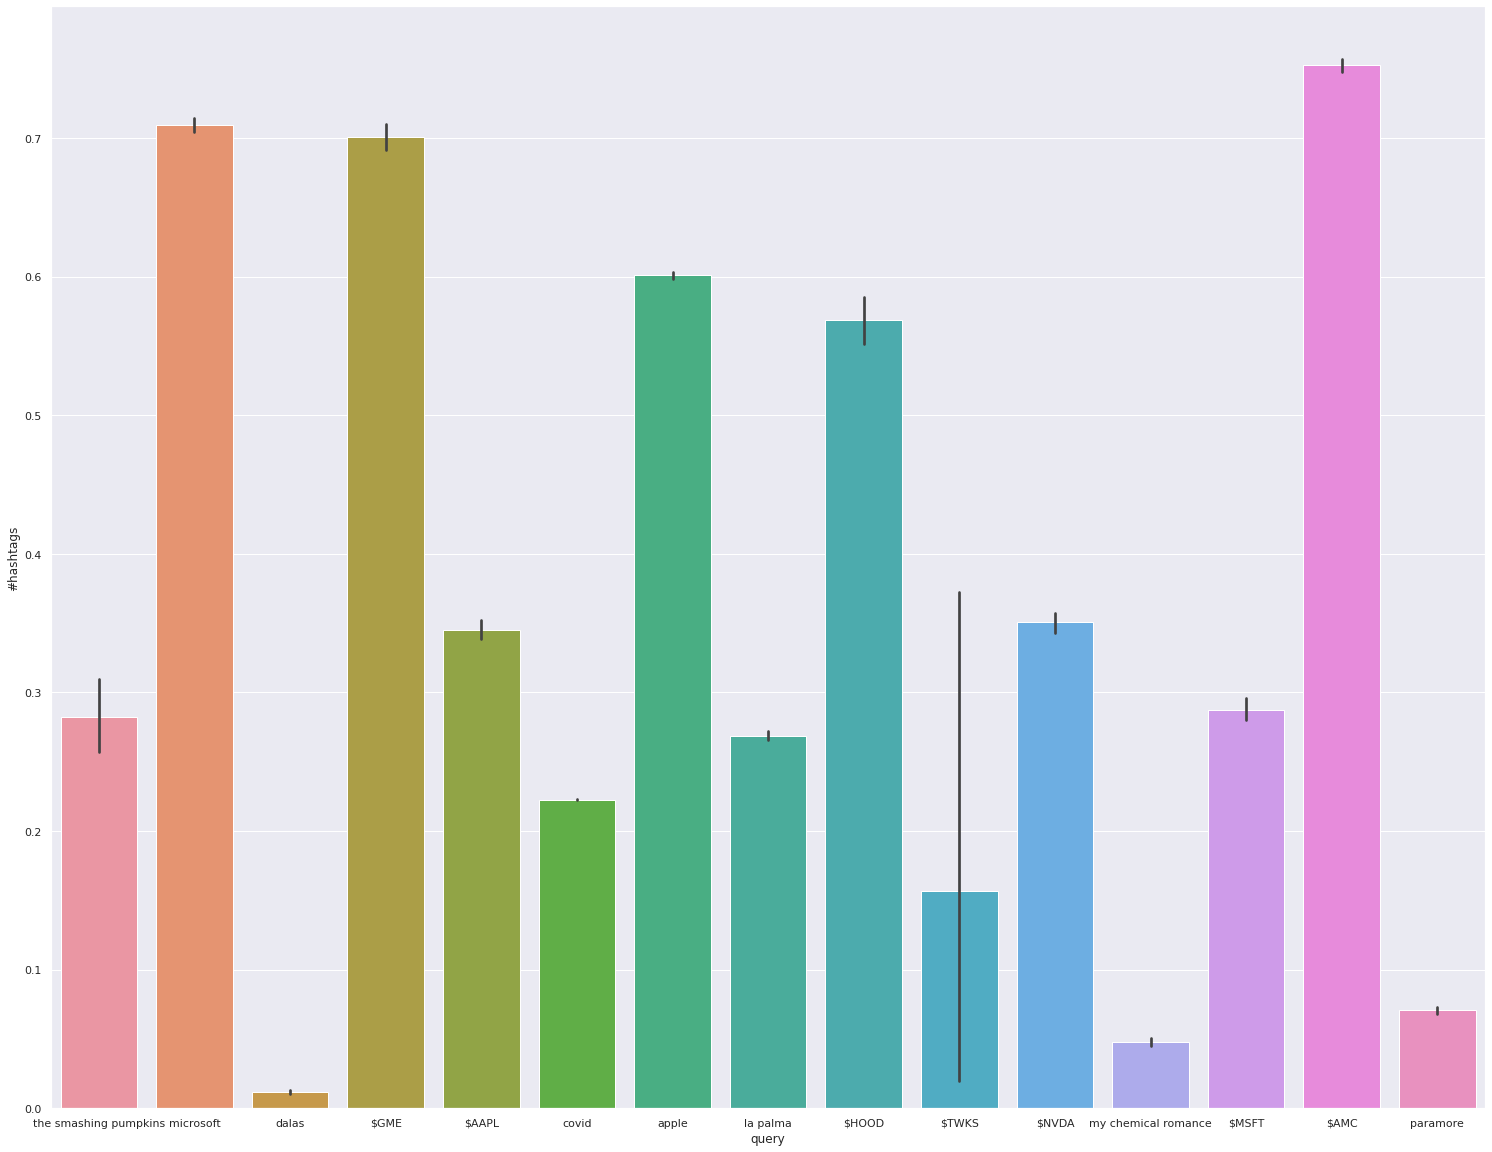
\includegraphics[scale=0.26]{twitter/namedentitylevel/twitter_averagecount_hashtags.png}
		\caption{Average number of hashtags per named entity.}
		\label{fig:twitter_averagecount_hashtags}
	\end{center}
\end{figure}

\par Lastly, a tweet may be a repost of other tweet. This is known as retweet and the number of retweets of a tweet could be a good indicator of its popularity. The Figure \ref{fig:twitter_counts_isrt} shows the number of tweets that are a retweet of other for each named entity. For the \textit{covid} keyword there are a large amount of retweets. However, for the remaining named entities, the number of tweets and retweets are similar.
\begin{figure}[H]
	\begin{center}
		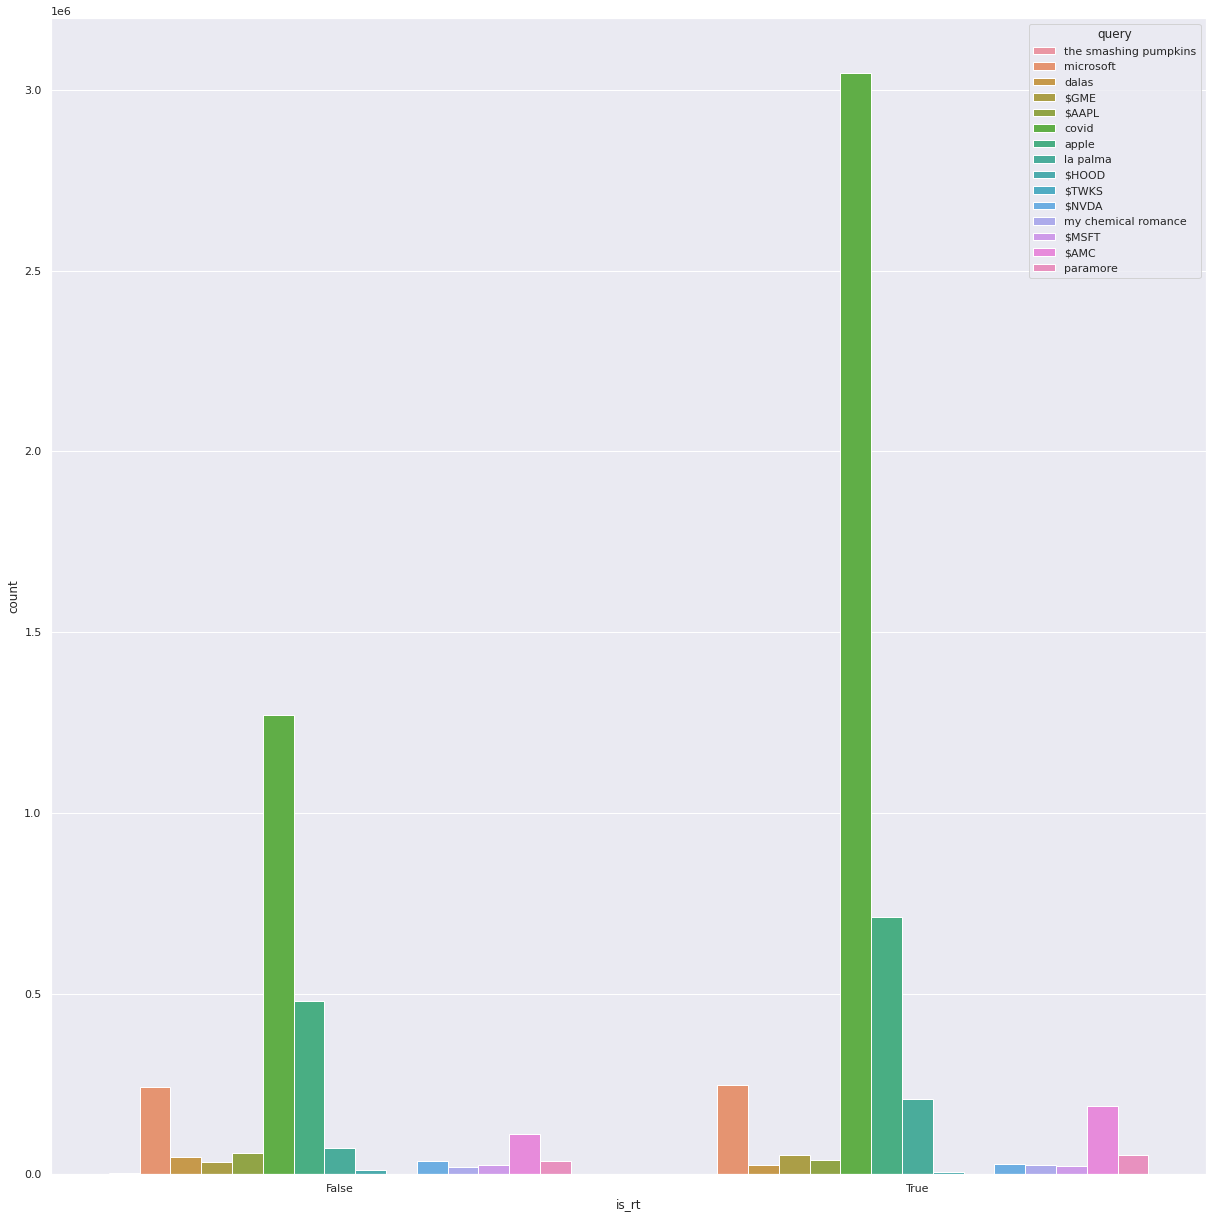
\includegraphics[scale=0.3]{twitter/namedentitylevel/twitter_counts_isrt.png}
		\caption{Count of tweets that are retweet per named entity.}
		\label{fig:twitter_counts_isrt}
	\end{center}
\end{figure}


\subsubsection{Blog posts named entity analysis}
For the blog posts dataset the average number of links per named entity is higher that the ones computed for the Twitter dataset. This reinforces the fact of using these links to enrich the textual data.

\begin{figure}[H]
	\begin{center}
		\includegraphics[scale=0.3]{blogposts/namedentitylevel/blogpost_average_\#links.png}
		\caption{Average number of links per named entity.}
		\label{fig:blogpost_average_links}
	\end{center}
\end{figure}

\par  The Figure \ref{fig:blogpost_average_tags_entity} plots the average number of tags per named entity. These values vary drastically compared to the averages computed for the Twitter dataset.
\begin{figure}[H]
	\begin{center}
		\includegraphics[scale=0.3]{blogposts/namedentitylevel/blogpost_average_\#tags.png}
		\caption{Average number of tags per named entity.}
		\label{fig:blogpost_average_tags_entity}
	\end{center}
\end{figure}

\par Finally, it seems that there are two predominant languages in this dataset since the number of blog posts written in English and Spanish for each named entity are greater than the number of posts for the remaining languages. The Figure \ref{fig:blogposts_postcount_lang_entity} depicts these statistics.
\begin{figure}[H]
	\begin{center}
		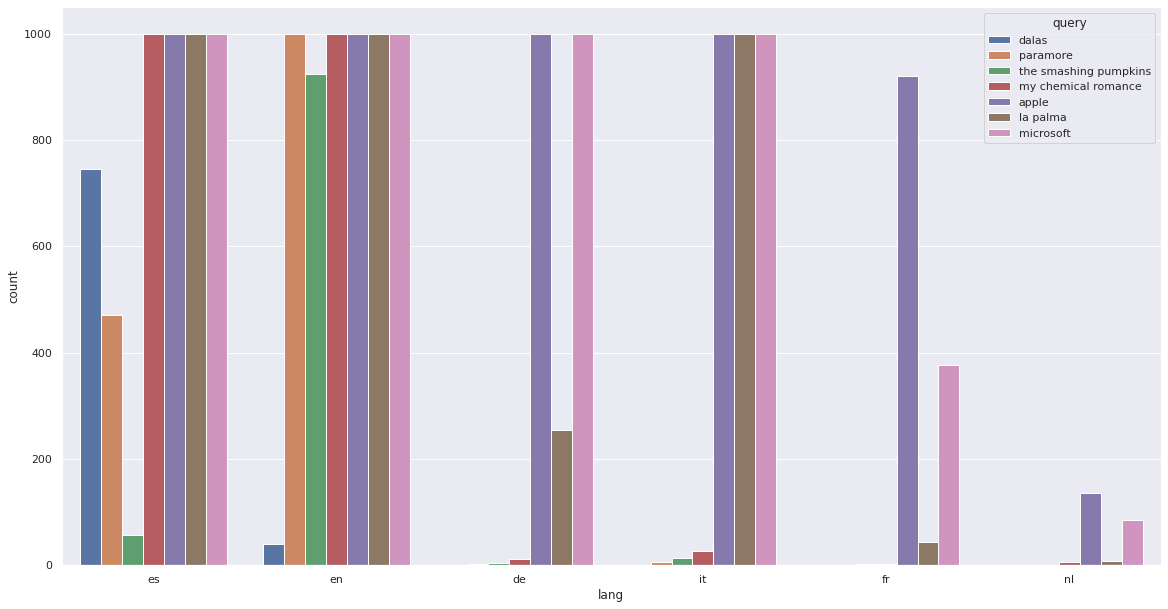
\includegraphics[scale=0.3]{blogposts/namedentitylevel/blogpost_postcount_lang.png}
		\caption{Blog posts count per language and named entity.}
		\label{fig:blogposts_postcount_lang_entity}
	\end{center}
\end{figure}



\subsubsection{Reddit named entity analysis}

\par Similar to the retweets, the number of comments and likes of a Reddit post could be a good indicator of popularity. The Figures \ref{fig:reddit_average_comments_entity} and \ref{fig:reddit_average_ups_entity} shows the average number of comments and likes per named entity. In general, the number of comments are similar except for the \textit{apple} and \textit{la palma} named entities.

\begin{figure}[H]
	\begin{center}
		\includegraphics[scale=0.3]{reddit/namedentitylevel/reddit_average_\#comments.png}
		\caption{Average number of comments per named entity.}
		\label{fig:reddit_average_comments_entity}
	\end{center}
\end{figure}

\begin{figure}[H]
	\begin{center}
		\includegraphics[scale=0.3]{reddit/namedentitylevel/reddit_average_\#ups.png}
		\caption{Reddit posts count per named entity.}
		\label{fig:reddit_average_ups_entity}
	\end{center}
\end{figure}

\par As expected, the number of Reddit posts in English is the biggest. However, it is interesting to remark that \textit{la palma} is a Spanish named entity. Despite of this, the number of posts in English containing this named entity are still greater than the number of posts for the Spanish language. 
\par Although in this work only five languages are considered, the Figure \ref{fig:reddit_postcount_lang_entity} shows other languages. This is due to issues of the Social Searcher API.
\begin{figure}[H]
	\begin{center}
		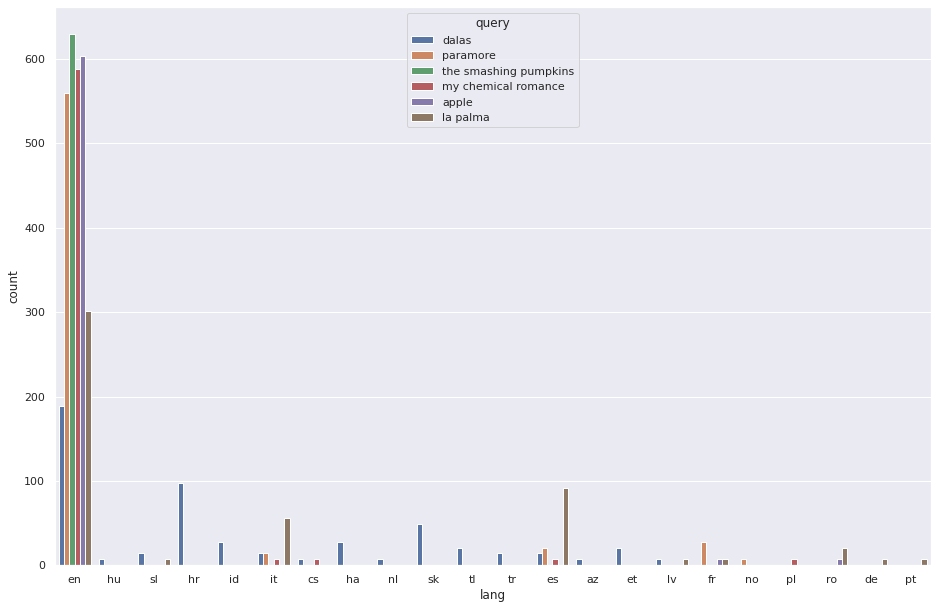
\includegraphics[scale=0.4]{reddit/namedentitylevel/reddit_postcount_lang.png}
		\caption{Blog posts count per language and named entity.}
		\label{fig:reddit_postcount_lang_entity}
	\end{center}
\end{figure}


\par Finally, the number of Reddit posts per sentiment and named entity is shown in the Figure \ref{fig:reddit_postcount_sentiment_entity}. The unbalancing of data with respect to this variable is not appropriate to train classifier models.
\begin{figure}[H]
	\begin{center}
		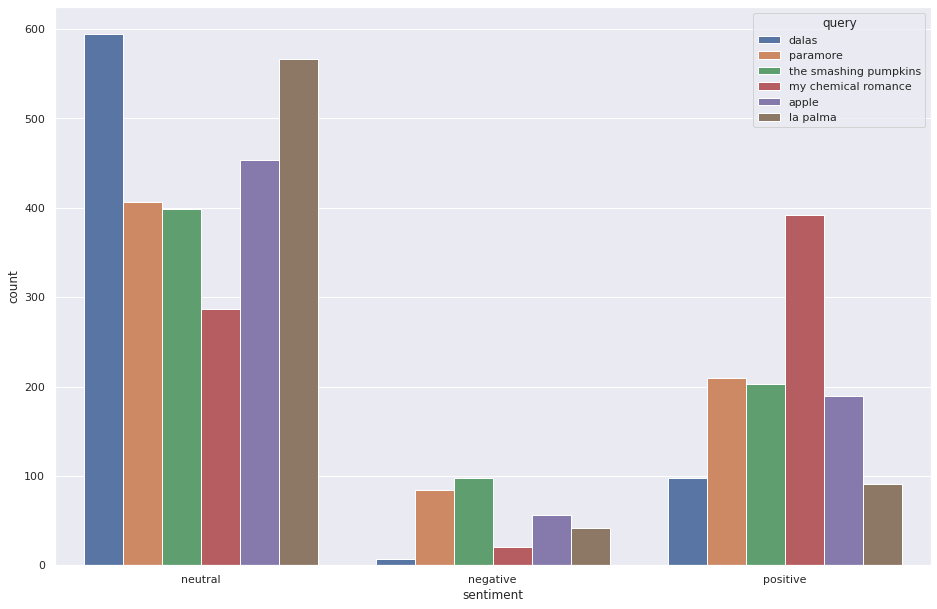
\includegraphics[scale=0.4]{reddit/namedentitylevel/reddit_postcount_sentiment.png}
		\caption{Reddit posts count per sentiment and named entity.}
		\label{fig:reddit_postcount_sentiment_entity}
	\end{center}
\end{figure}


\section{Adaptations of NLP tools}

The specific lingo used in social networks requires to readapt the current NLP tools in order to capture these nuances. Hashtags, abbreviations, misspellings, emoticons or inconsistent capitalization or punctuation must be taken into account by the already trained models. Current tokenizers must cover these patterns. \citep{Nikfarjam2015} coded regular expressions for tweets and reached a F-measure value of 0.96. However, to code manual rules implies that they probably will need to be reconsidered if the domain application is changed since they focused on tweets that mention drugs.
\par Part of speech taggers must face the out of vocabulary words (OOV) since the misspellings or short forms will be incorrectly classified by the current taggers. Hence, re-training the current models and extend the tag set is mandatory \citep{synthesisLecturesSocial}. \citep{stanfordTwitterPosTagger} proposes a system based con Conditional Random Fields and clustering OOV words to reach an accuracy value of 0.85 but they did not consider a including new tags in the tag set. \citep{gimpelPosSetExtended} extended the tag set for Twitter to cover hashtags, links, etc and obtained an accuracy value of 0.9. Likewise, chunkers and parsers must be reconditioned. \citep{khanParserAdaptation} proposes a dependency parser but was designed over specific Twitter dataset.
%Tokenizers: The specific ling
%TODO include captures
%TODO explain each one
% Copora analysis at dataset level
	% Number of posts of each social media
	% Number of posts of each language an social media
	% Distribution of links of each social media
	
% Corpora analysis at named entity level
	% Twitter 
		% # hashags containing the named entity
		% # links
		% # Rt's
		% Number of posts published per day
		
	% Reddit

		% average ups per entity (or box plot)
		% average comments per entity (or boxplot)
		% Number of negative and positive reddits posts
		% # posts per language
	%Twingly posts
		% Distribution of number of posts for each language
		% Distribution of number of posts with links
		% Number of posts published per day
		% Average number of tags
		% Average length of text and title
		% 
